\chapter{Data Pre-processing and Noise Handling}
\label{ch:pre}

The pipeline (implemented in \texttt{src/data\_radhar.py}, shared by both
datasets) is described below, technique by technique, in the
\emph{what / why / how / effect / limitation / verification} format.

\begin{figure}[h]
\centering
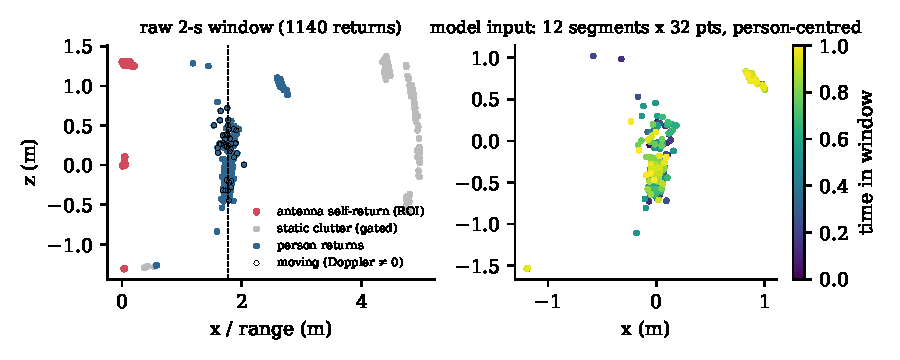
\includegraphics[width=\textwidth]{preproc_before_after.pdf}
\caption{One raw 2-s RadHAR window (left), with antenna self-returns (red),
static clutter removed by gating (grey), person returns (blue) and moving returns
(black circles), and the resulting model input (right).}
\label{fig:preprocreport}
\end{figure}

\section{Windowing}
\textbf{What:} 2-s windows (60 frames on RadHAR, 48 on MiliPoint) cut from one
recording or single-action run. \textbf{Why:} single frames hold only 6--21
returns and no motion information, and 2\,s matches the RadHAR protocol.
\textbf{How:} \texttt{make\_windows}; evaluation stride 10 frames (RadHAR) and 12
(MiliPoint); training stride 20 and 24, respectively. \textbf{Effect:} 3{,}565
RadHAR test windows (the original paper reports 3{,}538). \textbf{Limitation:}
activities shorter than 2\,s are not modelled. \textbf{Verification:} window
counts per split in the leakage audit.

\section{Region-of-interest (ROI) filter}
\textbf{What:} drop returns with $x<0.3$\,m (RadHAR only). \textbf{Why:} 34.6\% of
all returns are antenna self-reflections at $x\approx0$ (red points in
Fig.~\ref{fig:preprocreport}). \textbf{How:} \texttt{roi\_filter}. \textbf{Effect:}
these returns no longer distort the centroid or consume sampling slots.
\textbf{Limitation:} a person standing within 30\,cm of the radar would be
removed (an unrealistic set-up). \textbf{Verification:} EDA statistics.

\section{Person centring with moving returns}
\textbf{What:} express coordinates relative to the median of the window's
\emph{moving} returns (Doppler $\neq0$); fall back to the median of all returns.
\textbf{Why:} a plain centroid was pulled metres away by clutter (Issue \#13).
Static objects have zero radial velocity, whereas a performing person always
produces some moving returns. The median is robust to the remaining outliers.
\textbf{How:} \texttt{RadHARWindows.person\_centre}. \textbf{Effect:} translation
invariance with respect to where the person stands; removes distance as a cue.
\textbf{Limitation:} a motionless person has no moving returns (fallback used);
two moving people would be merged. \textbf{Verification:} ablation ``no centring''
was dropped for compute reasons. The gating ablation (below) covers the combined
effect.

\section{Spatial gating (clutter removal)}
\textbf{What:} drop returns more than 1.2\,m (horizontal distance) from the person
centre. \textbf{Why:} after the ROI filter, 50.1\% of returns are static clutter
clusters at 2.5\,m and 4.5\,m. Because training and test recordings share the
room, this clutter is also a potential scene \emph{shortcut}. \textbf{How:} applied
per segment before sampling. 1.2\,m covers arm span and in-place walking (the
median distance of returns from the centre is 0.9--1.6\,m before gating).
\textbf{Effect:} the sampled points come from the person. \textbf{Limitation:}
returns from limbs farther than 1.2\,m would be lost; the radius was chosen from
EDA, not tuned on test data. \textbf{Verification:} ablation \emph{-- spatial gating}
(Table~\ref{tab:ablation}).

\section{Temporal segmentation and point sampling}
\textbf{What:} split the window into $G=12$ segments and sample $P=32$ returns per
segment (with replacement if fewer). \textbf{Why:} a fixed tensor size is needed
for batching and edge inference; accumulating 4--5 frames per segment densifies
the cloud while keeping temporal order. \textbf{How:} \texttt{\_\_getitem\_\_};
evaluation uses a fixed per-sample seed so that test inputs are deterministic.
\textbf{Effect:} $12\times32\times6$ input. \textbf{Limitation:} duplicated points
when segments are sparse. \textbf{Verification:} unit test of shapes and
determinism.

\section{Feature normalisation}
Intensity is standardised with mean and standard deviation computed on the
\emph{training recordings only}. The validation and test sets reuse these values
(verified by the audit, Chapter~\ref{ch:leak}). Coordinates are already in
metres and person-centred. Time is normalised to $[0,1]$.

\section{Training-time augmentation}
\label{sec:aug}
\textbf{Standard (all models):} random rotation about the vertical axis
($\pm15^\circ$), isotropic scaling ($[0.9,1.1]$), 1-cm Gaussian jitter, and fresh
point sampling every epoch. \textbf{Noise-robust training (optional,
\texttt{--robust 1}):} per batch, each with probability 0.5: variable per-segment
density (keep 30--100\%), point dropout (0--20\%), false-detection injection
(0--10\% of returns), and with probability 0.25 the loss of one temporal segment.
All of these are applied to training batches only, from a separate random
generator (seeded $10{,}000+\mathrm{seed}$) that is never used at test time.

\section{Controlled noise conditions for evaluation}
Measured dataset noise (self-returns, clutter, sparsity) is handled by the
pre-processing above. To probe robustness beyond it, the \emph{test} inputs are
perturbed synthetically (\texttt{src/noise.py}), after pre-processing, with fixed
seeds so that every model sees identical perturbed samples
(Table~\ref{tab:noisecond}). These conditions are experimental manipulations,
not claims about the noise present in the datasets.

\begin{table}[h]
\centering
\caption{Evaluation perturbations (applied to the held-out test set only).}
\label{tab:noisecond}
\small
\begin{tabular}{L{2.6cm}L{6.2cm}L{4.6cm}}
\toprule
Condition & Operation & Levels \\
\midrule
Coordinate jitter & add $\mathcal{N}(0,\sigma^2)$ to $x,y,z$ & $\sigma=0.02, 0.05, 0.10$\,m \\
Point dropout & remove returns (slots masked, variable count) & 5, 15, 30\% \\
Increased sparsity & keep a fraction of unique returns, re-sample to $P$ & keep 50, 25, 12.5\% \\
Outlier injection & replace returns by uniform false detections in $\pm1.5$\,m & 5, 10, 20\% \\
Variable density & per-segment keep fraction $\sim U(k,1)$ & $k=0.5, 0.25, 0.1$ \\
Frame loss & drop whole temporal segments & 25, 50\% of segments \\
Combined & density + jitter + outliers + dropout & severity 1, 2, 3 \\
\bottomrule
\end{tabular}
\end{table}

\section{Methods investigated but not used}
Statistical and radius-based outlier removal and DBSCAN clustering were
considered. Gating around the moving-point centre removes the dominant clutter
with one interpretable parameter and no per-window clustering cost. Additional
filters on the remaining sparse body returns would risk removing limb points, so
they were not adopted. This decision was made from the EDA (the clutter forms
far-away clusters) and was not tuned on test data.
